\section{Non-crossing Partitions}

\begin{definition}[Non-crossing Partition]
    A \emph{non-crossing partition} of a \emph{totally
    ordered} set $E$ is
    a set partition $P = \{E_1, E_2, \ldots, E_k\}$ such that
    if $a, c \in E_i$, $b, d \in E_j$, and $i \neq j$, then
    we do \emph{not} have $a < b < c < d$, nor $a > b > c > d$.\\
    We denote by $\mathcal{NC}_n$ the set of non-crossing partitions
    of $\{1, 2, \ldots, n\}$.
    $$\mathcal{NC} = \bigcup_{n > 0}{\mathcal{NC}_n}$$
\end{definition}

From this point, we assume that every partition $P = \{B_1, \ldots, B_l\}$
is \emph{sorted} such that :\\
\begin{itemize*}
    \item For each block $B_i = \{b_1, \ldots, b_k\} \in P$,
        $b_1 < \ldots < b_k$\\
    \item $min (B_1) < \ldots < min (B_k)$\\
\end{itemize*}

\begin{notation}
    $[n] = \{1, 2, \ldots, n\}$
\end{notation}

\begin{example}[$E = \lbrack 6 \rbrack $]
    \begin{align*}
        &P_1 = \{\{1, 2, 5\}, \{3, 4\}, \{6\}\} \in \mathcal{NC}_6\\
        &P_2 = \{\{1, 2, 4\}, \{3, 5\}, \{6\}\} \notin \mathcal{NC}_6
    \end{align*}
\end{example}

\begin{theorem}
    Let $nc_n$ be the cardinal of $\mathcal{NC}_n$.
    We have $$nc_n = \frac{1}{n + 1} \binom{2n}{n}$$
    which is again the $n^{th}$ Catalan number
    $Cat(n)$.
\end{theorem}

\begin{example}[$n = 1, 2, 3$]
    ~\\
    \begin{itemize*}
        \item $n = 1$ \  $:$ \  $nc_1 = 1$\\
        \subitem $\{\{1\}\}$\\
        \item $n = 2$ \  $:$ \  $nc_2 = 2$\\
        \subitem $\{\{1, 2\}\}$
        \subitem $\{\{1\}, \{2\}\}$\\
        \item $n = 3$ \  $:$ \  $nc_3 = 5$\\
        \subitem $\{\{1, 2, 3\}\}$
        \subitem $\{\{1\}, \{2, 3\}\}$
        \subitem $\{\{1, 3\}, \{2\}\}$
        \subitem $\{\{1, 2\}, \{3\}\}$
        \subitem $\{\{1\}, \{2\}, \{3\}\}$\\
    \end{itemize*}
\end{example}

\begin{prop}
    This means we can create a \emph{bijection} between
    $\mathcal{PF'}_n$ and $\mathcal{NC}_n$.
\end{prop}

\begin{proof}
    ~\\
\begin{itemize}
    \item $\mathcal{NC}_n \to \mathcal{PF'}_n$ :
    For each block $B$ in the non-crossing partition, take
    $i = min (B)$, and let $k_i = size (B)$.\\
    $k_i = 0$ if $i$ is not the minimum of a block.\\
    The corresponding parking function is
    $(\underbrace{1, \ldots, 1}_{k_1}, \underbrace{2, \ldots,
    2}_{k_2}, \ldots, \underbrace{n, \ldots, n}_{k_n})$.\\
    \item $\mathcal{PF'}_n \to \mathcal{NC}_n$ :
    For each $i$ in $[n]$, if $i$ appears $n_i$ times in the
    parking function, $B_i$ will be of size $n_i$ with minimum
    element $i$.
    There is a unique set partition $\displaystyle P = \bigcup_{i}{B_i}$
    of $[n]$ respecting these conditions that is non-crossing :
    for each minimum $i$ in \emph{decreasing order}, add
    the $n_i$ first free elements of
    $[i+1, i+2, \ldots, n, 1, \ldots, i-1]$ to $B_i$.
\end{itemize}
\end{proof}

\begin{example}[$n = 6$]
    \begin{align*}
        &P = \{\{1, 2, 5\}, \{3, 4\}, \{6\}\}
        &f = (1, 1, 1, 3, 3, 6)\\
    \end{align*}
\end{example}

\begin{cor}
    A non-crossing partition can be represented by the minimums
    and sizes of its blocks.
\end{cor}

\begin{example}
    $\{\{1, 2, 5\}, \{3, 4\}, \{6\}\}$ can be represented by
    the following dictionnary :\\
    \begin{itemize*}
        \item 1 : 3\\
        \item 3 : 2\\
        \item 6 : 1\\
    \end{itemize*}
\end{example}

A non-crossing partition of $[n]$ can be represented graphically
on a regular $n$-vertices polygon, with vertices labeled from $1$
to $n$ clockwise. We then represent each block $B = \{b_1, \ldots, b_k\}$
by the convex hull of $\{b_1, \ldots, b_k\}$.\\

\begin{example}[$P = \{\{1, 2, 5\}, \{3, 4\}, \{6\}\}$]
    ~\\
\begin{center}
    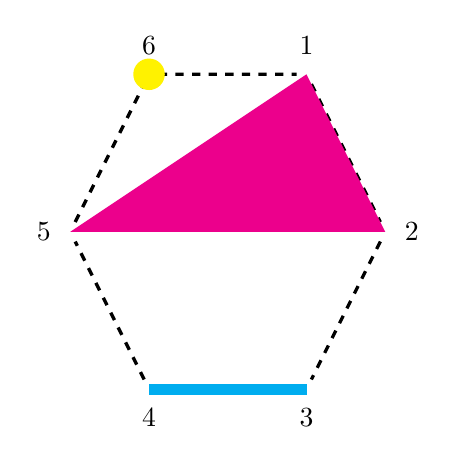
\begin{tikzpicture}[scale=1]
        \node [label = above : {$1$}] (1)
            at (4,5) {};
        \node [label = right : {$2$}] (2)
            at (5,3) {};
        \node [label = below : {$3$}] (3)
            at (4,1) {};
        \node [label = below : {$4$}] (4)
            at (2,1) {};
        \node [label = left : {$5$}]  (5)
            at (1,3) {};
        \node [label = above : {$6$}] (6)
            at (2,5) {};
        \draw [dashed][very thick]
        (1) -- (2) -- (3) -- (4)
            -- (5) -- (6) -- (1);
        \fill [color = magenta] (4,5) -- (5,3)
            -- (1,3) -- cycle;
        \draw [color = cyan][line width = 4pt] 
            (4,1) -- (2,1);
        \fill [color=yellow] (2,5) circle (0.2);
      \end{tikzpicture}
\end{center}
    Thus non-crossing meaning the hulls are
    \emph{disjoint}.\\
\end{example}

\begin{example}[Counter-example : $P = \{\{1, 5, 2\},
    \{3, 6\}, \{4\}\}$]
    \begin{center}
    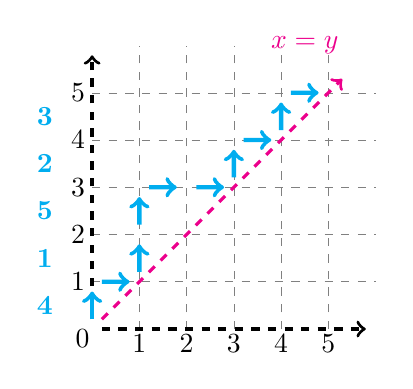
\begin{tikzpicture}[scale=0.6]
        \node (a) at (0, 0) {};
        \node (b) at (0, 6) {};
        \node (c) at (6, 0) {};
        \node (d) at (5.5, 5.5) {};

        \draw [dashed, very thin, color=gray] (1,0) to (1,6);
        \draw [dashed, very thin, color=gray] (2,0) to (2,6);
        \draw [dashed, very thin, color=gray] (3,0) to (3,6);
        \draw [dashed, very thin, color=gray] (4,0) to (4,6);
        \draw [dashed, very thin, color=gray] (5,0) to (5,6);
        \draw [dashed, very thin, color=gray] (0,1) to (6,1);
        \draw [dashed, very thin, color=gray] (0,2) to (6,2);
        \draw [dashed, very thin, color=gray] (0,3) to (6,3);
        \draw [dashed, very thin, color=gray] (0,4) to (6,4);
        \draw [dashed, very thin, color=gray] (0,5) to (6,5);

        \node (e) at (4.5, 6) [color = magenta] {$x = y$}; 
        \draw [dashed, very thick, ->] (a) to (b);
        \draw [dashed, very thick, ->] (a) to (c);
        \draw [dashed, very thick, ->]
            [color = magenta] (a) to (d);

        \node (1)  at (0,0)   {};
        \node (2)  at (0,1)   {};
        \node (3)  at (1,1)   {};
        \node (4)  at (1,2)   {};
        \node (5)  at (1,3)   {};
        \node (6)  at (2,3)   {};
        \node (7)  at (3,3)   {};
        \node (8)  at (3,4)   {};
        \node (9)  at (4,4)   {};
        \node (10) at (4,5)   {};
        \node (11) at (5,5)   {};
        \draw [->, ultra thick, color = cyan]
            (1)  to (2);
        \draw [->, ultra thick, color = cyan] 
            (2)  to (3);
        \draw [->, ultra thick, color = cyan]
            (3)  to (4);
        \draw [->, ultra thick, color = cyan]
            (4)  to (5);
        \draw [->, ultra thick, color = cyan]
            (5)  to (6);
        \draw [->, ultra thick, color = cyan]
            (6)  to (7);
        \draw [->, ultra thick, color = cyan]
            (7)  to (8);
        \draw [->, ultra thick, color = cyan]
            (8)  to (9);
        \draw [->, ultra thick, color = cyan]
            (9)  to (10);
        \draw [->, ultra thick, color = cyan]
            (10) to (11);

        \node at (-0.2, -0.2) {$0$};
        \node at (-0.3, 1)    {$1$};
        \node at (1, -0.3)    {$1$};
        \node at (-0.3, 2)    {$2$};
        \node at (2, -0.3)    {$2$};
        \node at (-0.3, 3)    {$3$};
        \node at (3, -0.3)    {$3$};
        \node at (-0.3, 4)    {$4$};
        \node at (4, -0.3)    {$4$};
        \node at (-0.3, 5)    {$5$};
        \node at (5, -0.3)    {$5$};

        \node [color = cyan] at (-1, 0.5) {\textbf{4}};
        \node [color = cyan] at (-1, 1.5) {\textbf{1}};
        \node [color = cyan] at (-1, 2.5) {\textbf{5}};
        \node [color = cyan] at (-1, 3.5) {\textbf{2}};
        \node [color = cyan] at (-1, 4.5) {\textbf{3}};

    \end{tikzpicture}
\end{center}
    This partition is \emph{not} non-crossing, as the
    convex hulls of $\{1, 2, 5\}$ and $\{3, 6\}$ are
    \emph{not} disjoint.
\end{example}

\subsection{The non-crossing partitions poset}

\begin{definition}[$\succ$]
    We say that $P$ covers $Q$, written $P \succ Q$,
    if $\exists B_i, B_j \in P$ such that
    $Q = P - \{B_i, B_j\} \cup \{B_i \cup B_j\}$    
\end{definition}

\begin{example}
    $\{\{1, 6\}, \{2, 3\}, \{4, 5\}\} \succ
    \{\{1, 2, 3, 6\}, \{4, 5\}\}$\\
    \begin{itemize*}
        \item $B_i = \{1, 6\}$\\
        \item $B_j = \{2, 3\}$\\
    \end{itemize*}
\end{example}

\begin{prop}
    This covering relation defines the \emph{poset}
    of $\mathcal{NC}_n$.
    We denote by $\mathcal{NCC}_n$ the set of
    \emph{maximal chains} in the poset of $\mathcal{NC}_n$.\\
    $$\mathcal{NCC} = \bigcup_{n > 0}{\mathcal{NCC}_n}$$
\end{prop}

\begin{rem}
    The bottom element of this poset is $\{\{1, \ldots, n\}\}$,
    and the top element is $\{\{1\}, \ldots, \{n\}\}$.
\end{rem}

\begin{theorem}
    Let $ncc_n$ be the cardinal of $\mathcal{NCC}_n$.
    We have $$ncc_n = n^{n - 2}$$.
\end{theorem}

\begin{example}[The poset of $\mathcal{NC}_4$]
    ~\\
    To shorten labels, we represent $\{\{1\}, \{2, 3\},
    \{4\}\}$ by $1|23|4$. \\

    \begin{center}
        \begin{center}
    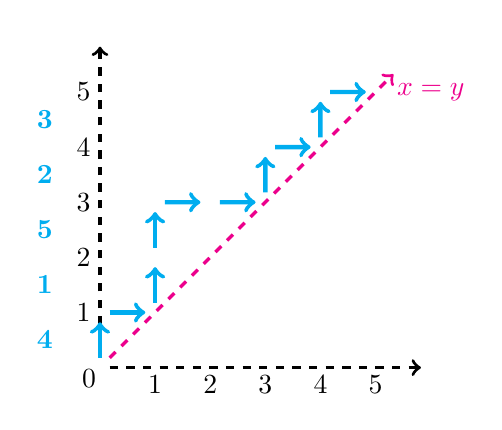
\begin{tikzpicture}[scale=0.7]
        \node (a) at (0, 0) {};
        \node (b) at (0, 6) {};
        \node (c) at (6, 0) {};
        \node (d) at (5.5, 5.5) {};
        \node (e) at (6, 5) [color = magenta]
            {$x = y$}; 
        \draw [dashed, very thick, ->] (a) to (b);
        \draw [dashed, very thick, ->] (a) to (c);
        \draw [dashed, very thick, ->]
            [color = magenta] (a) to (d);

        \node (1)  at (0,0)   {};
        \node (2)  at (0,1)   {};
        \node (3)  at (1,1)   {};
        \node (4)  at (1,2)   {};
        \node (5)  at (1,3)   {};
        \node (6)  at (2,3)   {};
        \node (7)  at (3,3)   {};
        \node (8)  at (3,4)   {};
        \node (9)  at (4,4)   {};
        \node (10) at (4,5)   {};
        \node (11) at (5,5)   {};
        \draw [->, ultra thick, color = cyan]
            (1)  to (2);
        \draw [->, ultra thick, color = cyan] 
            (2)  to (3);
        \draw [->, ultra thick, color = cyan]
            (3)  to (4);
        \draw [->, ultra thick, color = cyan]
            (4)  to (5);
        \draw [->, ultra thick, color = cyan]
            (5)  to (6);
        \draw [->, ultra thick, color = cyan]
            (6)  to (7);
        \draw [->, ultra thick, color = cyan]
            (7)  to (8);
        \draw [->, ultra thick, color = cyan]
            (8)  to (9);
        \draw [->, ultra thick, color = cyan]
            (9)  to (10);
        \draw [->, ultra thick, color = cyan]
            (10) to (11);

        \node at (-0.2, -0.2) {$0$};
        \node at (-0.3, 1)    {$1$};
        \node at (1, -0.3)    {$1$};
        \node at (-0.3, 2)    {$2$};
        \node at (2, -0.3)    {$2$};
        \node at (-0.3, 3)    {$3$};
        \node at (3, -0.3)    {$3$};
        \node at (-0.3, 4)    {$4$};
        \node at (4, -0.3)    {$4$};
        \node at (-0.3, 5)    {$5$};
        \node at (5, -0.3)    {$5$};

        \node [color = cyan] at (-1, 0.5) {\textbf{4}};
        \node [color = cyan] at (-1, 1.5) {\textbf{1}};
        \node [color = cyan] at (-1, 2.5) {\textbf{5}};
        \node [color = cyan] at (-1, 3.5) {\textbf{2}};
        \node [color = cyan] at (-1, 4.5) {\textbf{3}};

    \end{tikzpicture}
\end{center}
        There are $4^2 = 16$ different maximal chains,
        and $\frac {1}{5} \binom{8}{4} = \frac{70}{5} = 14$
        elements in this poset.
    \end{center}
\end{example}


\subsection{Kreweras complement}

\begin{definition}[Associated Permutation]
    The \emph{permutation} $\sigma$ associated to a non-crossing
    partition has a cycle $(b_1, \ldots, b_k)$ for each block
    $B = \{b_1, \ldots, b_k\}$ of the partition.
\end{definition}

\begin{example}
    The permutation associated to $\{\{1, 2, 5\}, \{3, 4\}, \{6\}\}$
    is $(1\ 2\ 5)\ (3\ 4)\ (6) = 254316$.
\end{example}

\begin{definition}[Kreweras Complement]
    The \emph{Kreweras complement} $K (P)$ of a non-crossing
    partition $P$ is defined as follows :\\
    \begin{itemize*}
        \item Let $\sigma$ be the permutation associated to $P$\\
        \item Let $\pi$ be the permutation $(n\ n-1\ n-2\
        \ldots\ 3\ 2\ 1) = n123 \ldots n-1$\\
        \item $K (P)$ is the \emph{non-crossing partition}
        associated to $\pi \sigma$.\\
    \end{itemize*}
\end{definition}

\begin{example}[$P = \{\{1, 2, 5\}, \{3, 4\}, \{6\}\}$]
    ~\\
    \begin{itemize*}
        \item $\sigma = (1\ 2\ 5)\ (3\ 4)\ (6) = 254316$\\
        \item $\pi = (6\ 5\ 4\ 3\ 2\ 1) = 612345$\\
        \item $\pi \sigma = 143265 = (1)\ (2\ 4)\ (3)\ (5\ 6)$\\
        \item $K(P) = \{\{1\},\{2, 4\}, \{3\}, \{5, 6\}\}$\\
    \end{itemize*}
\end{example}

\begin{prop}[Kreweras minimums]
        Let $P = \{B_1, \ldots, B_k\}$ be a non-crossing partition.
        Let $K (P) = \{B'_1, \ldots, B'_l\}$ be its Kreweras complement.
        Then $$\bigcup_{1 \leq i \leq l}{min (B'_i)} =
        B_1 \cup \bigcup_{1 < j \leq k}{B_i - {max (B_i)}}$$\\
\end{prop}

\begin{example}[$P = \{\{1, 2, 5\}, \{3, 4\}, \{6\}\}$]
    ~\\
    \begin{itemize}
        \item $K (P) = \{\{1\},\{2, 4\}, \{3\}, \{5, 6\}\}$
        \item $\bigcup{min (B'_i)} = \{1, 2, 3, 5\}$
        \item $B_1\ \cup\ \bigcup{B_i - {max (B_i)}}
        = \{1, 2, 5\} \cup \{3, 4\} - \{4\} \cup \{6\} - \{6\}
        = \{1, 2, 5\} \cup \{3\} \cup \emptyset = \{1, 2, 3, 5\}$\\
    \end{itemize}
\end{example}

\begin{notation}
    $B_{[i]} = $ block containing $i$.
\end{notation}

\begin{prop}[Kreweras block sizes]
    Let $P = \{B_1, \ldots, B_k\}$ be a non-crossing partition.
    Let $K (P) = \{B'_1, \ldots, B'_l\}$ be its Kreweras complement.
    Then the size of the block $B'_i$ is defined as follows :
    \begin{itemize}
        \item Let $m_i$ be the the $i^{th}$ minimum of $K (P)$
        \item Define a \emph{transition} $\phi (e)$ as 
            \subitem Let $j = e + 1$ (or $1$ if $e = n$)
            \subitem $\phi(e) = max (B_{[j]})$
        \item The size of $B'_i$ is $k_{min}$ such that
        $k_{min} = min \{k > 0\ |\ \phi^k (m_i) \in B_{[m_i]}\}$.\\
    \end{itemize}
\end{prop}

\begin{example}[$P = \{\{1, 2, 5\}, \{3, 4\}, \{6\}\}$]
    ~\\
    \begin{itemize}
        \item $mins = \{1, 2, 3, 5\}$
        \item $m_1 = 1$
            \subitem $B_{[1]} = B_1$
            \subitem $max (B_{[2]} = max (B_1) = 5$
            \subitem The size for $m_1$ is $1$.
        \item $m_2$
            \subitem $B_{[2]} = B_1$
            \subitem $max (B_{[3]}) = max (B_2) = 4$
            \subitem $max (B_{[5]}) = max (B_1) = 5$
            \subitem The size for $m_2$ is $2$.
        \item $m_3 = 3$
            \subitem $B_{[3]} = B_2$
            \subitem $max (B_{[4]}) = max (B_2) = 4$
            \subitem The size for $m_3$ is $1$.
        \item $m_4 = 5$
            \subitem $B_{[5]} = B_1$
            \subitem $max (B_{[6]}) = max (B_3) = 6$
            \subitem $max (B_{[1]}) = max (B_1) = 5$
            \subitem The size for $m_4$ is $2$.
    \end{itemize}
\end{example}

\begin{definition}[Mutually Non-crossing Partitions]
    2 partitions $P$ and $Q$ are said
    \emph{mutually non-crossing} if :\\
    \begin{itemize*}
        \item P is non-crossing\\
        \item Q is non-crossing\\
        \item For every block $B_i$ of $P$ and every
        block $B_j$ of $Q$, if $a,c \in B_i$ and
        $b, d \in B_j$, then we can \emph{not} have
        $a < b < c < d$, nor $a > b > c > d$.
    \end{itemize*}    
\end{definition}

\begin{example}[$P = \{\{1, 2\},\{3, 6\},\ \{4, 5\}\},
    Q = \{\{1, 6\}, \{2\}, \{3, 4\}, \{5\}\}$]
        \begin{center}
        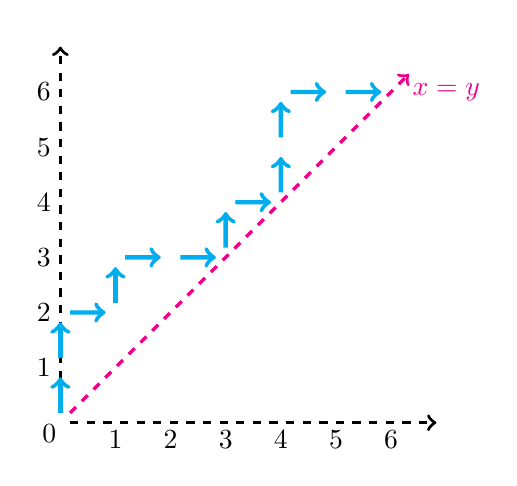
\begin{tikzpicture}[scale=0.7]
            \node (a) at (0, 0) {};
            \node (b) at (0, 7) {};
            \node (c) at (7, 0) {};
            \node (d) at (6.5, 6.5) {};
            \node (e) at (7, 6) [color = magenta]
                {$x = y$}; 
            \draw [dashed, very thick, ->] (a) to (b);
            \draw [dashed, very thick, ->] (a) to (c);
            \draw [dashed, very thick, ->]
                [color = magenta] (a) to (d);

            \node (1)  at (0,0)   {};
            \node (2)  at (0,1)   {};
            \node (3)  at (0,2)   {};
            \node (4)  at (1,2)   {};
            \node (5)  at (1,3)   {};
            \node (6)  at (2,3)   {};
            \node (7)  at (3,3)   {};
            \node (8)  at (3,4)   {};
            \node (9)  at (4,4)   {};
            \node (10) at (4,5)   {};
            \node (11) at (4,6)   {};
            \node (12) at (5,6)   {};
            \node (13) at (6,6)   {};
            \draw [->, ultra thick, color = cyan]
                (1)  to (2);
            \draw [->, ultra thick, color = cyan] 
                (2)  to (3);
            \draw [->, ultra thick, color = cyan]
                (3)  to (4);
            \draw [->, ultra thick, color = cyan]
                (4)  to (5);
            \draw [->, ultra thick, color = cyan]
                (5)  to (6);
            \draw [->, ultra thick, color = cyan]
                (6)  to (7);
            \draw [->, ultra thick, color = cyan]
                (7)  to (8);
            \draw [->, ultra thick, color = cyan]
                (8)  to (9);
            \draw [->, ultra thick, color = cyan]
                (9)  to (10);
            \draw [->, ultra thick, color = cyan]
                (10) to (11);
            \draw [->, ultra thick, color = cyan]
                (11) to (12);
            \draw [->, ultra thick, color = cyan]
                (12) to (13);

            \node at (-0.2, -0.2) {$0$};
            \node at (-0.3, 1)    {$1$};
            \node at (1, -0.3)    {$1$};
            \node at (-0.3, 2)    {$2$};
            \node at (2, -0.3)    {$2$};
            \node at (-0.3, 3)    {$3$};
            \node at (3, -0.3)    {$3$};
            \node at (-0.3, 4)    {$4$};
            \node at (4, -0.3)    {$4$};
            \node at (-0.3, 5)    {$5$};
            \node at (5, -0.3)    {$5$};
            \node at (-0.3, 6)    {$6$};
            \node at (6, -0.3)    {$6$};

        \end{tikzpicture}
    \end{center}
\end{example}

\begin{example}[Counter-example : $P = \{\{1, 2\},
    \{3, 6\},\ \{4, 5\}\},
    Q = \{\{1, 6\}, \{2, 5\}, \{3, 4\}\}$]
    
    \begin{center}
        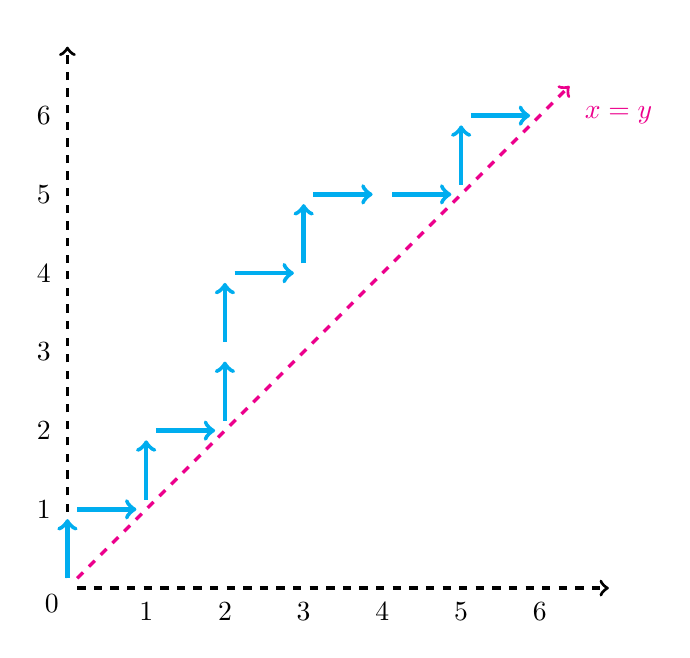
\begin{tikzpicture}[scale=1]
            \node (a) at (0, 0) {};
            \node (b) at (0, 7) {};
            \node (c) at (7, 0) {};
            \node (d) at (6.5, 6.5) {};
            \node (e) at (7, 6) [color = magenta]
                {$x = y$}; 
            \draw [dashed, very thick, ->] (a) to (b);
            \draw [dashed, very thick, ->] (a) to (c);
            \draw [dashed, very thick, ->]
                [color = magenta] (a) to (d);

            \node (1)  at (0,0)   {};
            \node (2)  at (0,1)   {};
            \node (3)  at (1,1)   {};
            \node (4)  at (1,2)   {};
            \node (5)  at (2,2)   {};
            \node (6)  at (2,3)   {};
            \node (7)  at (2,4)   {};
            \node (8)  at (3,4)   {};
            \node (9)  at (3,5)   {};
            \node (10) at (4,5)   {};
            \node (11) at (5,5)   {};
            \node (12) at (5,6)   {};
            \node (13) at (6,6)   {};
            \draw [->, ultra thick, color = cyan]
                (1)  to (2);
            \draw [->, ultra thick, color = cyan] 
                (2)  to (3);
            \draw [->, ultra thick, color = cyan]
                (3)  to (4);
            \draw [->, ultra thick, color = cyan]
                (4)  to (5);
            \draw [->, ultra thick, color = cyan]
                (5)  to (6);
            \draw [->, ultra thick, color = cyan]
                (6)  to (7);
            \draw [->, ultra thick, color = cyan]
                (7)  to (8);
            \draw [->, ultra thick, color = cyan]
                (8)  to (9);
            \draw [->, ultra thick, color = cyan]
                (9)  to (10);
            \draw [->, ultra thick, color = cyan]
                (10) to (11);
            \draw [->, ultra thick, color = cyan]
                (11) to (12);
            \draw [->, ultra thick, color = cyan]
                (12) to (13);

            \node at (-0.2, -0.2) {$0$};
            \node at (-0.3, 1)    {$1$};
            \node at (1, -0.3)    {$1$};
            \node at (-0.3, 2)    {$2$};
            \node at (2, -0.3)    {$2$};
            \node at (-0.3, 3)    {$3$};
            \node at (3, -0.3)    {$3$};
            \node at (-0.3, 4)    {$4$};
            \node at (4, -0.3)    {$4$};
            \node at (-0.3, 5)    {$5$};
            \node at (5, -0.3)    {$5$};
            \node at (-0.3, 6)    {$6$};
            \node at (6, -0.3)    {$6$};

        \end{tikzpicture}
    \end{center}
\end{example}

\begin{rem}
    Note that vertices \emph{can} touch, but the edges
    of the convex hulls can \emph{not} cross.
\end{rem}

\begin{prop}
    For any non-crossing partition $P$, $P$ and $K(P)$
    are mutually non-crossing.\\
    Furthermore, $K(P)$ is a \emph{densest} partition that
    is mutually non-crossing with $P$. That is, \emph{no}
    partition $Q$ that is mutually non-crossing with $P$
    has less blocks than $K(P)$.
\end{prop}

\begin{example}[$P = \{1, 2, 6\}, \{3, 5\}, \{4\}\}$]
    $Q = \{\{1\}, \{2, 5\}, \{3, 4\}, \{6\}\}$
    \begin{center}
    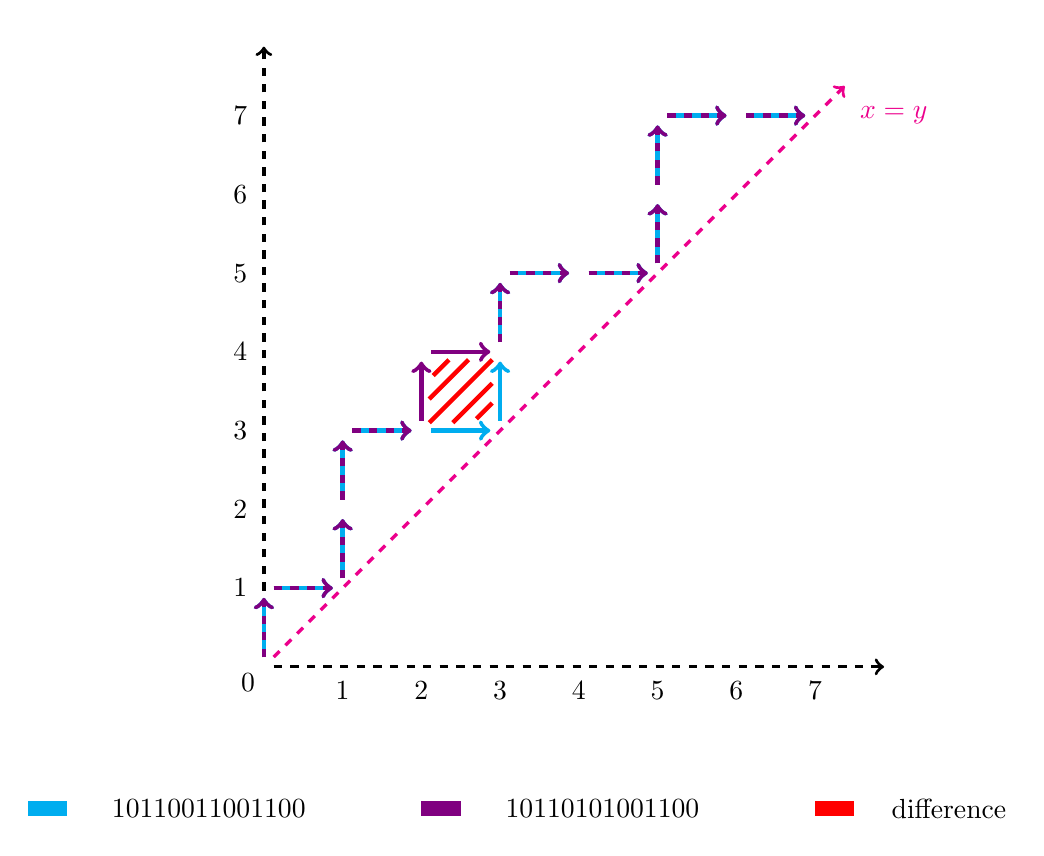
\begin{tikzpicture}[scale=1]
        \node (a) at (0, 0) {};
        \node (b) at (0, 8) {};
        \node (c) at (8, 0) {};
        \node (d) at (7.5, 7.5) {};
        \node (e) at (8, 7) [color = magenta]
            {$x = y$}; 
        \draw [dashed, very thick, ->] (a) to (b);
        \draw [dashed, very thick, ->] (a) to (c);
        \draw [dashed, very thick, ->]
            [color = magenta] (a) to (d);

        \node (1)  at (0,0)   {};
        \node (2)  at (0,1)   {};
        \node (3)  at (1,1)   {};
        \node (4)  at (1,2)   {};
        \node (5)  at (1,3)   {};
        \node (6)  at (2,3)   {};
        \node (7)  at (3,3)   {};
        \node (7b) at (2,4)   {};
        \node (8)  at (3,4)   {};
        \node (9)  at (3,5)   {};
        \node (10) at (4,5)   {};
        \node (11) at (5,5)   {};
        \node (12) at (5,6)   {};
        \node (13) at (5,7)   {};
        \node (14) at (6,7)   {};
        \node (15) at (7,7)   {};

        \draw [->, ultra thick, color = cyan]
            (1)  to (2);
        \draw [->, ultra thick, color = cyan] 
            (2)  to (3);
        \draw [->, ultra thick, color = cyan]
            (3)  to (4);
        \draw [->, ultra thick, color = cyan]
            (4)  to (5);
        \draw [->, ultra thick, color = cyan]
            (5)  to (6);
        \draw [->, ultra thick, color = cyan]
            (6)  to (7);
        \draw [->, ultra thick, color = cyan]
            (7)  to (8);
        \draw [->, ultra thick, color = cyan]
            (8)  to (9);
        \draw [->, ultra thick, color = cyan]
            (9)  to (10);
        \draw [->, ultra thick, color = cyan]
            (10) to (11);
        \draw [->, ultra thick, color = cyan]
            (11) to (12);
        \draw [->, ultra thick, color = cyan]
            (12) to (13);
        \draw [->, ultra thick, color = cyan]
            (13) to (14);
        \draw [->, ultra thick, color = cyan]
            (14) to (15);

        \draw [->, dashed, ultra thick, color = violet]
            (1)  to (2);
        \draw [->, dashed, ultra thick, color = violet] 
            (2)  to (3);
        \draw [->, dashed, ultra thick, color = violet]
            (3)  to (4);
        \draw [->, dashed, ultra thick, color = violet]
            (4)  to (5);
        \draw [->, dashed, ultra thick, color = violet]
            (5)  to (6);
        \draw [->, ultra thick, color = violet]
            (6)  to (7b);
        \draw [->, ultra thick, color = violet]
            (7b)  to (8);
        \draw [->, dashed, ultra thick, color = violet]
            (8)  to (9);
        \draw [->, dashed, ultra thick, color = violet]
            (9)  to (10);
        \draw [->, dashed, ultra thick, color = violet]
            (10) to (11);
        \draw [->, dashed, ultra thick, color = violet]
            (11) to (12);
        \draw [->, dashed, ultra thick, color = violet]
            (12) to (13);
        \draw [->, dashed, ultra thick, color = violet]
            (13) to (14);
        \draw [->, dashed, ultra thick, color = violet]
            (14) to (15);

        \node at (-0.2, -0.2) {$0$};
        \node at (-0.3, 1)    {$1$};
        \node at (1, -0.3)    {$1$};
        \node at (-0.3, 2)    {$2$};
        \node at (2, -0.3)    {$2$};
        \node at (-0.3, 3)    {$3$};
        \node at (3, -0.3)    {$3$};
        \node at (-0.3, 4)    {$4$};
        \node at (4, -0.3)    {$4$};
        \node at (-0.3, 5)    {$5$};
        \node at (5, -0.3)    {$5$};
        \node at (-0.3, 6)    {$6$};
        \node at (6, -0.3)    {$6$};
        \node at (-0.3, 7)    {$7$};
        \node at (7, -0.3)    {$7$};

        \draw[color = red, ultra thick]
            (2.1,3.1) -- (2.9,3.9);
        \draw[color = red, ultra thick]
            (2.1,3.4) -- (2.6,3.9);
        \draw[color = red, ultra thick]
            (2.15,3.7) -- (2.35,3.9);
        \draw[color = red, ultra thick]
            (2.4,3.1) -- (2.9,3.6);
        \draw[color = red, ultra thick]
            (2.7,3.15) -- (2.9,3.35);

        \fill[color = cyan] (-3,-1.9) rectangle
            (-2.5,-1.7);
        \node at (-0.7,-1.8) {$10110011001100$};
        \fill[color = violet] (2,-1.9) rectangle
        (2.5,-1.7);
        \node at (4.3,-1.8) {$10110101001100$};
        \fill[color = red] (7,-1.9) rectangle
        (7.5,-1.7);
        \node at (8.7,-1.8) {difference};
    \end{tikzpicture}
\end{center}
\end{example}

\subsection{Action of $\mathfrak{S}_n$ on partitions of 
$[n]$}

\begin{definition}[Action of $\mathfrak{S}_n$]
    The action of $\mathfrak{S}_n$ on a partition
    $P = \{B_1, \ldots, B_l\}$ of $[n]$ is defined by :\\
    \begin{itemize*}
        \item For each block $B_i = \{b_1, \ldots, b_k\}$ :
        $\sigma(Bi) =\{\sigma (b_1), \ldots, \sigma (b_k)\}$ \\
        \item When $P \in \mathcal{NC}_n$, we denote 
        $\rho = \sigma(P) =
            \{\sigma (B_1), \ldots, \sigma (B_l)\}$
    \end{itemize*}
\end{definition}

\begin{example}[$\sigma = 415362,
    P = \{\{1, 6\}, \{2, 3, 5\}, \{4\}\}$]
    ~\\
    $\sigma (P) = 
        \{\{1, 5, 6\}, \{2, 4\}, \{3\}\}$
        ~\\
    \begin{center}
        \begin{center}
    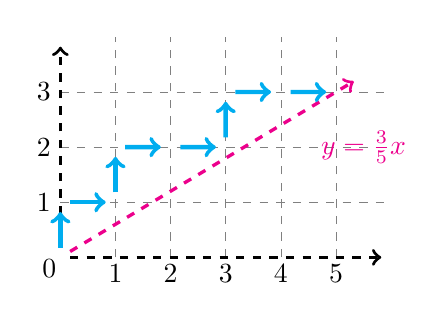
\begin{tikzpicture}[scale=0.7]
        \node (a) at (0, 0) {};
        \node (b) at (0, 4) {};
        \node (c) at (6, 0) {};
        \node (d) at (5.5, 3.3) {};

        \draw [dashed, very thin, color=gray] (1,0) to (1,4);
        \draw [dashed, very thin, color=gray] (2,0) to (2,4);
        \draw [dashed, very thin, color=gray] (3,0) to (3,4);
        \draw [dashed, very thin, color=gray] (4,0) to (4,4);
        \draw [dashed, very thin, color=gray] (5,0) to (5,4);
        \draw [dashed, very thin, color=gray] (0,1) to (6,1);
        \draw [dashed, very thin, color=gray] (0,2) to (6,2);
        \draw [dashed, very thin, color=gray] (0,3) to (6,3);
        
        \node (e) at (5.5, 2) [color = magenta] {$y = \frac{3}{5}x$}; 
        \draw [dashed, very thick, ->] (a) to (b);
        \draw [dashed, very thick, ->] (a) to (c);
        \draw [dashed, very thick, ->]
            [color = magenta] (a) to (d);

        \node (1)  at (0,0)   {};
        \node (2)  at (0,1)   {};
        \node (3)  at (1,1)   {};
        \node (4)  at (1,2)   {};
        \node (5)  at (2,2)   {};
        \node (6)  at (3,2)   {};
        \node (7)  at (3,3)   {};
        \node (8)  at (4,3)   {};
        \node (9)  at (5,3)   {};
        \draw [->, ultra thick, color = cyan]
            (1)  to (2);
        \draw [->, ultra thick, color = cyan] 
            (2)  to (3);
        \draw [->, ultra thick, color = cyan]
            (3)  to (4);
        \draw [->, ultra thick, color = cyan]
            (4)  to (5);
        \draw [->, ultra thick, color = cyan]
            (5)  to (6);
        \draw [->, ultra thick, color = cyan]
            (6)  to (7);
        \draw [->, ultra thick, color = cyan]
            (7)  to (8);
        \draw [->, ultra thick, color = cyan]
            (8)  to (9);

        \node at (-0.2, -0.2) {$0$};
        \node at (-0.3, 1)    {$1$};
        \node at (1, -0.3)    {$1$};
        \node at (-0.3, 2)    {$2$};
        \node at (2, -0.3)    {$2$};
        \node at (-0.3, 3)    {$3$};
        \node at (3, -0.3)    {$3$};
        \node at (4, -0.3)    {$4$};
        \node at (5, -0.3)    {$5$};

    \end{tikzpicture}
\end{center}
        \begin{center}
    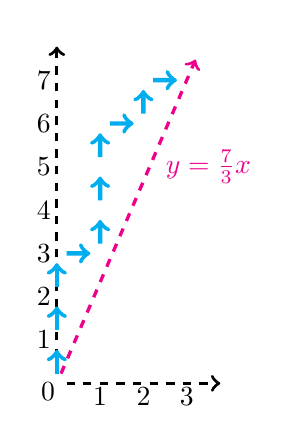
\begin{tikzpicture}[scale=0.55]
        \node (a) at (0, 0) {};
        \node (b) at (0, 8) {};
        \node (c) at (4, 0) {};
        \node (d) at (3.3, 7.7) {};
        \node (e) at (3.5, 5) [color = magenta]
            {$y = \frac{7}{3}x$}; 
        \draw [dashed, very thick, ->] (a) to (b);
        \draw [dashed, very thick, ->] (a) to (c);
        \draw [dashed, very thick, ->]
            [color = magenta] (a) to (d);

        \node (1)  at (0,0)   {};
        \node (2)  at (0,1)   {};
        \node (3)  at (0,2)   {};
        \node (4)  at (0,3)   {};
        \node (5)  at (1,3)   {};
        \node (6)  at (1,4)   {};
        \node (7)  at (1,5)   {};
        \node (8)  at (1,6)   {};
        \node (9)  at (2,6)   {};
        \node (10) at (2,7)   {};
        \node (11) at (3,7)   {};
        \draw [->, ultra thick, color = cyan]
            (1)  to (2);
        \draw [->, ultra thick, color = cyan] 
            (2)  to (3);
        \draw [->, ultra thick, color = cyan]
            (3)  to (4);
        \draw [->, ultra thick, color = cyan]
            (4)  to (5);
        \draw [->, ultra thick, color = cyan]
            (5)  to (6);
        \draw [->, ultra thick, color = cyan]
            (6)  to (7);
        \draw [->, ultra thick, color = cyan]
            (7)  to (8);
        \draw [->, ultra thick, color = cyan]
            (8)  to (9);
        \draw [->, ultra thick, color = cyan]
            (9)  to (10);
        \draw [->, ultra thick, color = cyan]
            (10) to (11);

        \node at (-0.2, -0.2) {$0$};
        \node at (-0.3, 1)    {$1$};
        \node at (1, -0.3)    {$1$};
        \node at (-0.3, 2)    {$2$};
        \node at (2, -0.3)    {$2$};
        \node at (-0.3, 3)    {$3$};
        \node at (3, -0.3)    {$3$};
        \node at (-0.3, 4)    {$4$};
        \node at (-0.3, 5)    {$5$};
        \node at (-0.3, 6)    {$6$};
        \node at (-0.3, 7)    {$7$};

    \end{tikzpicture}
\end{center}
    \end{center}
\end{example}

\begin{rem}
    Note that $\mathcal{NC}_n$ is \emph{not} stable under
    the action of $\mathfrak{S}_n$.
    That is, even if $P$ is non-crossing, $\sigma (P)$ is 
    \emph{not} necessarily non-crossing.
\end{rem}

\begin{example}[Counter-example : $\sigma = 413562,
    P = \{\{1, 6\}, \{2, 3, 5\}, \{4\}\}$]
    $\sigma (P) = 
        \{\{1, 3, 6\}, \{2, 4\}, \{5\}\}$
        ~\\
    \begin{center}
        \begin{center}
    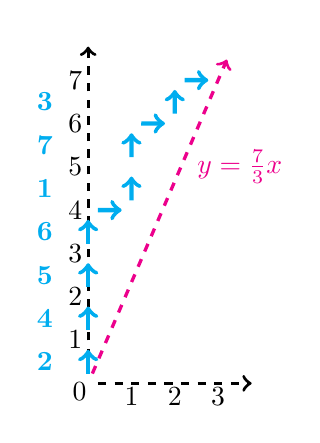
\begin{tikzpicture}[scale=0.55]
        \node (a) at (0, 0) {};
        \node (b) at (0, 8) {};
        \node (c) at (4, 0) {};
        \node (d) at (3.3, 7.7) {};
        \node (e) at (3.5, 5) [color = magenta]
            {$y = \frac{7}{3}x$}; 
        \draw [dashed, very thick, ->] (a) to (b);
        \draw [dashed, very thick, ->] (a) to (c);
        \draw [dashed, very thick, ->]
            [color = magenta] (a) to (d);

        \node (1)  at (0,0)   {};
        \node (2)  at (0,1)   {};
        \node (3)  at (0,2)   {};
        \node (4)  at (0,3)   {};
        \node (5)  at (0,4)   {};
        \node (6)  at (1,4)   {};
        \node (7)  at (1,5)   {};
        \node (8)  at (1,6)   {};
        \node (9)  at (2,6)   {};
        \node (10) at (2,7)   {};
        \node (11) at (3,7)   {};
        \draw [->, ultra thick, color = cyan]
            (1)  to (2);
        \draw [->, ultra thick, color = cyan] 
            (2)  to (3);
        \draw [->, ultra thick, color = cyan]
            (3)  to (4);
        \draw [->, ultra thick, color = cyan]
            (4)  to (5);
        \draw [->, ultra thick, color = cyan]
            (5)  to (6);
        \draw [->, ultra thick, color = cyan]
            (6)  to (7);
        \draw [->, ultra thick, color = cyan]
            (7)  to (8);
        \draw [->, ultra thick, color = cyan]
            (8)  to (9);
        \draw [->, ultra thick, color = cyan]
            (9)  to (10);
        \draw [->, ultra thick, color = cyan]
            (10) to (11);

        \node at (-0.2, -0.2) {$0$};
        \node at (-0.3, 1)    {$1$};
        \node at (1, -0.3)    {$1$};
        \node at (-0.3, 2)    {$2$};
        \node at (2, -0.3)    {$2$};
        \node at (-0.3, 3)    {$3$};
        \node at (3, -0.3)    {$3$};
        \node at (-0.3, 4)    {$4$};
        \node at (-0.3, 5)    {$5$};
        \node at (-0.3, 6)    {$6$};
        \node at (-0.3, 7)    {$7$};

        \node [color = cyan] at (-1, 0.5) {\textbf{2}};
        \node [color = cyan] at (-1, 1.5) {\textbf{4}};
        \node [color = cyan] at (-1, 2.5) {\textbf{5}};
        \node [color = cyan] at (-1, 3.5) {\textbf{6}};
        \node [color = cyan] at (-1, 4.5) {\textbf{1}};
        \node [color = cyan] at (-1, 5.5) {\textbf{7}};
        \node [color = cyan] at (-1, 6.5) {\textbf{3}};
    \end{tikzpicture}
\end{center}
        \begin{center}
    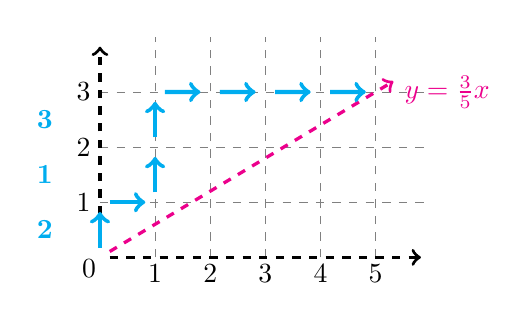
\begin{tikzpicture}[scale=0.7]
        \node (a) at (0, 0) {};
        \node (b) at (0, 4) {};
        \node (c) at (6, 0) {};
        \node (d) at (5.5, 3.3) {};

        \draw [dashed, very thin, color=gray] (1,0) to (1,4);
        \draw [dashed, very thin, color=gray] (2,0) to (2,4);
        \draw [dashed, very thin, color=gray] (3,0) to (3,4);
        \draw [dashed, very thin, color=gray] (4,0) to (4,4);
        \draw [dashed, very thin, color=gray] (5,0) to (5,4);
        \draw [dashed, very thin, color=gray] (0,1) to (6,1);
        \draw [dashed, very thin, color=gray] (0,2) to (6,2);
        \draw [dashed, very thin, color=gray] (0,3) to (6,3);

        \node (e) at (6.3, 3) [color = magenta] {$y = \frac{3}{5}x$}; 
        \draw [dashed, very thick, ->] (a) to (b);
        \draw [dashed, very thick, ->] (a) to (c);
        \draw [dashed, very thick, ->]
            [color = magenta] (a) to (d);

        \node (1)  at (0,0)   {};
        \node (2)  at (0,1)   {};
        \node (3)  at (1,1)   {};
        \node (4)  at (1,2)   {};
        \node (5)  at (1,3)   {};
        \node (6)  at (2,3)   {};
        \node (7)  at (3,3)   {};
        \node (8)  at (4,3)   {};
        \node (9)  at (5,3)   {};
        \draw [->, ultra thick, color = cyan]
            (1)  to (2);
        \draw [->, ultra thick, color = cyan] 
            (2)  to (3);
        \draw [->, ultra thick, color = cyan]
            (3)  to (4);
        \draw [->, ultra thick, color = cyan]
            (4)  to (5);
        \draw [->, ultra thick, color = cyan]
            (5)  to (6);
        \draw [->, ultra thick, color = cyan]
            (6)  to (7);
        \draw [->, ultra thick, color = cyan]
            (7)  to (8);
        \draw [->, ultra thick, color = cyan]
            (8)  to (9);

        \node at (-0.2, -0.2) {$0$};
        \node at (-0.3, 1)    {$1$};
        \node at (1, -0.3)    {$1$};
        \node at (-0.3, 2)    {$2$};
        \node at (2, -0.3)    {$2$};
        \node at (-0.3, 3)    {$3$};
        \node at (3, -0.3)    {$3$};
        \node at (4, -0.3)    {$4$};
        \node at (5, -0.3)    {$5$};

        \node [color = cyan] at (-1, 0.5) {\textbf{2}};
        \node [color = cyan] at (-1, 1.5) {\textbf{1}};
        \node [color = cyan] at (-1, 2.5) {\textbf{3}};
    \end{tikzpicture}
\end{center}
    \end{center}
\end{example}

\begin{definition}[Rotation]
    We define the \emph{rotation operator} $rot$ of
    $P \in \mathcal{NC}_n$ as $rot (P) = 
    (1\ 2\ 3\  \ldots \ n)(P) = 23 \ldots n1 (P)$.\\
    Conversely, we define $rot^{-1}$ of $P$ as
    $rot^{-1}(P) = (n\ n-1\ \ldots 3\ 2\ 1)(P) = 
    n12 \ldots n-1 (P)$.
\end{definition}

\begin{example}[$P = \{\{1, 6\}, \{2, 3, 5\}, \{4\}\}$]
    ~
    \begin{itemize}
        \item $rot (P) = \{\{1, 2\}, \{3, 4, 6\}, \{5\}\}$
        \item $rot^{-1}(P) = \{\{1, 2, 4\}, \{3\}, \{5, 6\}\}$
    \end{itemize}
    \begin{center}
        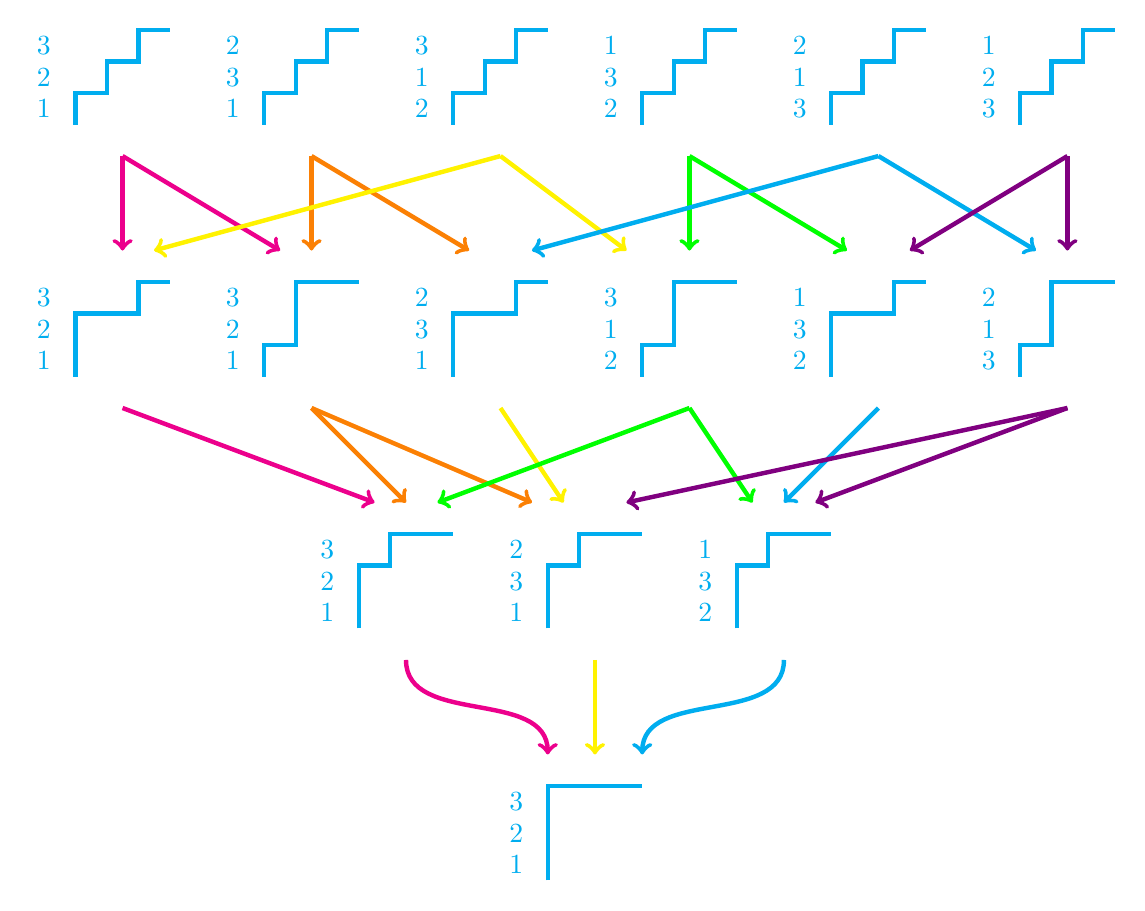
\begin{tikzpicture}[scale = 0.4]
    \draw [ultra thick, color = cyan] (0,0) -- (0,1)
        -- (0,2) -- (0,3) -- (1,3) -- (2,3) -- (3,3);
    \node[color = cyan] at (-1,0.5) {$1$};
    \node[color = cyan] at (-1,1.5) {$2$};
    \node[color = cyan] at (-1,2.5) {$3$};

    \draw [ultra thick, color = cyan] (-6,8) -- (-6,9)
        -- (-6,10) -- (-5,10) -- (-5,11) -- (-4,11)
        -- (-3,11);
    \node[color = cyan] at (-7,8.5) {$1$};
    \node[color = cyan] at (-7,9.5) {$2$};
    \node[color = cyan] at (-7,10.5) {$3$};
        
    \draw [ultra thick, color = cyan] (0,8) -- (0,9)
        -- (0,10) -- (1,10) -- (1,11) -- (2,11)
        -- (3,11);
    \node[color = cyan] at (-1,8.5) {$1$};
    \node[color = cyan] at (-1,9.5) {$3$};
    \node[color = cyan] at (-1,10.5) {$2$};

    \draw [ultra thick, color = cyan] (6,8) -- (6,9)
        -- (6,10) -- (7,10) -- (7,11) -- (8,11)
         -- (9,11);
    \node[color = cyan] at (5,8.5) {$2$};
    \node[color = cyan] at (5,9.5) {$3$};
    \node[color = cyan] at (5,10.5) {$1$};

    \draw [ultra thick, color = cyan] (-15,16) -- (-15,17)
        -- (-15,18) -- (-14,18) -- (-13,18) -- (-13,19)
        -- (-12,19);
    \node[color = cyan] at (-16,16.5) {$1$};
    \node[color = cyan] at (-16,17.5) {$2$};
    \node[color = cyan] at (-16,18.5) {$3$};

    \draw [ultra thick, color = cyan] (-9,16) -- (-9,17)
        -- (-8,17) -- (-8,18) -- (-8,19) -- (-7,19)
        -- (-6,19);
    \node[color = cyan] at (-10,16.5) {$1$};
    \node[color = cyan] at (-10,17.5) {$2$};
    \node[color = cyan] at (-10,18.5) {$3$};

    \draw [ultra thick, color = cyan] (-3,16) -- (-3,17)
        -- (-3,18) -- (-2,18) -- (-1,18) -- (-1,19)
        -- (0,19);
    \node[color = cyan] at (-4,16.5) {$1$};
    \node[color = cyan] at (-4,17.5) {$3$};
    \node[color = cyan] at (-4,18.5) {$2$};

    \draw [ultra thick, color = cyan] (3,16) -- (3,17)
        -- (4,17) -- (4,18) -- (4,19) -- (5,19)
        -- (6,19);
    \node[color = cyan] at (2,16.5) {$2$};
    \node[color = cyan] at (2,17.5) {$1$};
    \node[color = cyan] at (2,18.5) {$3$};

    \draw [ultra thick, color = cyan] (9,16) -- (9,17)
        -- (9,18) -- (10,18) -- (11,18) -- (11,19)
        -- (12,19);
    \node[color = cyan] at (8,16.5) {$2$};
    \node[color = cyan] at (8,17.5) {$3$};
    \node[color = cyan] at (8,18.5) {$1$};

    \draw [ultra thick, color = cyan] (15,16) -- (15,17)
        -- (16,17) -- (16,18) -- (16,19) -- (17,19)
        -- (18,19);
    \node[color = cyan] at (14,16.5) {$3$};
    \node[color = cyan] at (14,17.5) {$1$};
    \node[color = cyan] at (14,18.5) {$2$};

    \draw [ultra thick, color = cyan] (-15,24) -- (-15,25)
        -- (-14,25) -- (-14,26) -- (-13,26) -- (-13,27)
        -- (-12,27);
    \node[color = cyan] at (-16,24.5) {$1$};
    \node[color = cyan] at (-16,25.5) {$2$};
    \node[color = cyan] at (-16,26.5) {$3$};

    \draw [ultra thick, color = cyan] (-9,24) -- (-9,25)
        -- (-8,25) -- (-8,26) -- (-7,26) -- (-7,27)
        -- (-6,27);
    \node[color = cyan] at (-10,24.5) {$1$};
    \node[color = cyan] at (-10,25.5) {$3$};
    \node[color = cyan] at (-10,26.5) {$2$};

    \draw [ultra thick, color = cyan] (-3,24) -- (-3,25)
        -- (-2,25) -- (-2,26) -- (-1,26) -- (-1,27)
        -- (0,27);
    \node[color = cyan] at (-4,24.5) {$2$};
    \node[color = cyan] at (-4,25.5) {$1$};
    \node[color = cyan] at (-4,26.5) {$3$};


    \draw [ultra thick, color = cyan] (3,24) -- (3,25)
        -- (4,25) -- (4,26) -- (5,26) -- (5,27)
        -- (6,27);
    \node[color = cyan] at (2,24.5) {$2$};
    \node[color = cyan] at (2,25.5) {$3$};
    \node[color = cyan] at (2,26.5) {$1$};

    \draw [ultra thick, color = cyan] (9,24) -- (9,25)
        -- (10,25) -- (10,26) -- (11,26) -- (11,27)
        -- (12,27);
    \node[color = cyan] at (8,24.5) {$3$};
    \node[color = cyan] at (8,25.5) {$1$};
    \node[color = cyan] at (8,26.5) {$2$};

    \draw [ultra thick, color = cyan] (15,24) -- (15,25)
        -- (16,25) -- (16,26) -- (17,26) -- (17,27)
        -- (18,27);
    \node[color = cyan] at (14,24.5) {$3$};
    \node[color = cyan] at (14,25.5) {$2$};
    \node[color = cyan] at (14,26.5) {$1$};

    \draw [->][color=magenta, ultra thick]
        (-13.5,23) to (-13.5,20);
    \draw [->][color=magenta, ultra thick]
        (-13.5,23) to (-8.5,20);
    \draw [->][color=magenta, ultra thick]
        (-13.5,15) to (-5.5,12); 
    \draw [->][out=-90,in=90, ultra thick] 
        [color=magenta](-4.5,7) to (0,4);

    \draw [->][color=brown!7!orange, ultra thick]
        (-7.5,23) to (-7.5,20);
    \draw [->][color=brown!7!orange, ultra thick]
        (-7.5,23) to (-2.5,20);
    \draw [->][color=brown!7!orange, ultra thick]
        (-7.5,15) to (-4.5,12);
    \draw [->][color=brown!7!orange, ultra thick]
        (-7.5,15) to (-0.5,12);

    \draw [->][color=yellow, ultra thick]
        (-1.5,23) to (-12.5,20);
    \draw [->][color=yellow, ultra thick]
        (-1.5,23) to (2.5,20);
    \draw [->][color=yellow, ultra thick]
        (-1.5,15) to (0.5,12); 
    \draw [->][out=-90,in=90, ultra thick] 
        [color=yellow](1.5,7) to (1.5,4);

    \draw [->][color = green,  ultra thick]
        (4.5,23) to (4.5,20);
    \draw [->][color=green, ultra thick]
        (4.5,23) to (9.5,20);
    \draw [->][color=green, ultra thick]
        (4.5,15) to (-3.5,12);
    \draw [->][color=green, ultra thick]
        (4.5,15) to (6.5,12);

    \draw [->][color=cyan, ultra thick]
        (10.5,23) to (-0.5,20);
    \draw [->][color=cyan, ultra thick]
        (10.5,23) to (15.5,20);
    \draw [->][color=cyan, ultra thick]
        (10.5,15) to (7.5,12); 
    \draw [->][out=-90,in=90, ultra thick] 
        [color=cyan](7.5,7) to (3,4);

    \draw [->][color=violet, ultra thick]
        (16.5,23) to (11.5,20);
    \draw [->][color=violet, ultra thick]
        (16.5,23) to (16.5,20);
    \draw [->][color=violet, ultra thick]
        (16.5,15) to (2.5,12);
    \draw [->][color=violet, ultra thick]
        (16.5,15) to (8.5,12);

\end{tikzpicture}

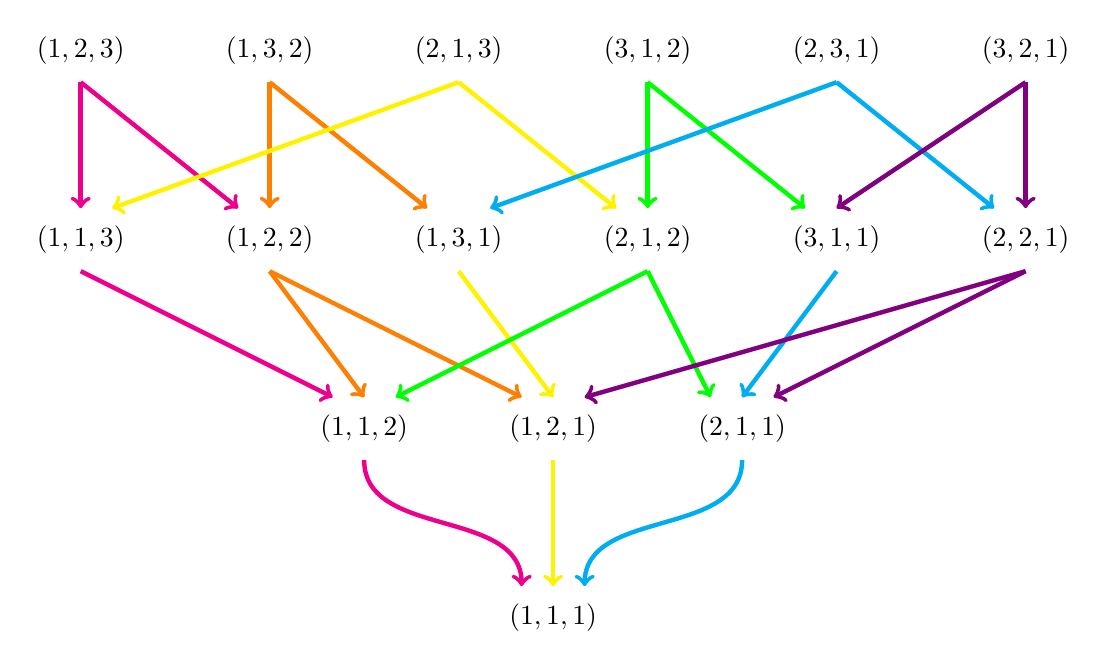
\begin{tikzpicture}[scale = 0.4]
    \node at (0,0) {$(1,1,1)$};

    \node at (-6,6) {$(1,1,2)$};                
    \node at (0,6)  {$(1,2,1)$};
    \node at (6,6)  {$(2,1,1)$};

    \node at (-15,12) {$(1,1,3)$};
    \node at (-9,12)  {$(1,2,2)$};
    \node at (-3,12)  {$(1,3,1)$};
    \node at (3,12)   {$(2,1,2)$};
    \node at (9,12)   {$(3,1,1)$};
    \node at (15,12)  {$(2,2,1)$};

    \node at (-15,18) {$(1,2,3)$};
    \node at (-9,18)  {$(1,3,2)$};
    \node at (-3,18)  {$(2,1,3)$};
    \node at (3,18)   {$(3,1,2)$};
    \node at (9,18)   {$(2,3,1)$};
    \node at (15,18)  {$(3,2,1)$};

    \draw [->][color=magenta, ultra thick]
        (-15,17) to (-15,13);
    \draw [->][color=magenta, ultra thick]
        (-15,17) to (-10,13);
    \draw [->][color=magenta, ultra thick]
        (-15,11) to (-7,7); 
    \draw [->][out=-90,in=90, ultra thick] 
        [color=magenta](-6,5) to (-1,1);

    \draw [->][color=brown!7!orange, ultra thick]
        (-9,17) to (-9,13);
    \draw [->][color=brown!7!orange, ultra thick]
        (-9,17) to (-4,13);
    \draw [->][color=brown!7!orange, ultra thick]
        (-9,11) to (-6,7);
    \draw [->][color=brown!7!orange, ultra thick]
        (-9,11) to (-1,7);

    \draw [->][color=yellow, ultra thick]
        (-3,17) to (-14,13);
    \draw [->][color=yellow, ultra thick]
        (-3,17) to (2,13);
    \draw [->][color=yellow, ultra thick]
        (-3,11) to (0,7); 
    \draw [->][out=-90,in=90, ultra thick] 
        [color=yellow](0,5) to (0,1);

    \draw [->][color = green,  ultra thick]
        (3,17) to (3,13);
    \draw [->][color=green, ultra thick]
        (3,17) to (8,13);
    \draw [->][color=green, ultra thick]
        (3,11) to (-5,7);
    \draw [->][color=green, ultra thick]
        (3,11) to (5,7);

    \draw [->][color=cyan, ultra thick]
        (9,17) to (-2,13);
    \draw [->][color=cyan, ultra thick]
        (9,17) to (14,13);
    \draw [->][color=cyan, ultra thick]
        (9,11) to (6,7); 
    \draw [->][out=-90,in=90, ultra thick] 
        [color=cyan](6,5) to (1,1);

    \draw [->][color=violet, ultra thick]
        (15,17) to (9,13);
    \draw [->][color=violet, ultra thick]
        (15,17) to (15,13);
    \draw [->][color=violet, ultra thick]
        (15,11) to (1,7);
    \draw [->][color=violet, ultra thick]
        (15,11) to (7,7);

\end{tikzpicture}
~\\
~\\
      ~\\
      ~\\
        
\begin{center}
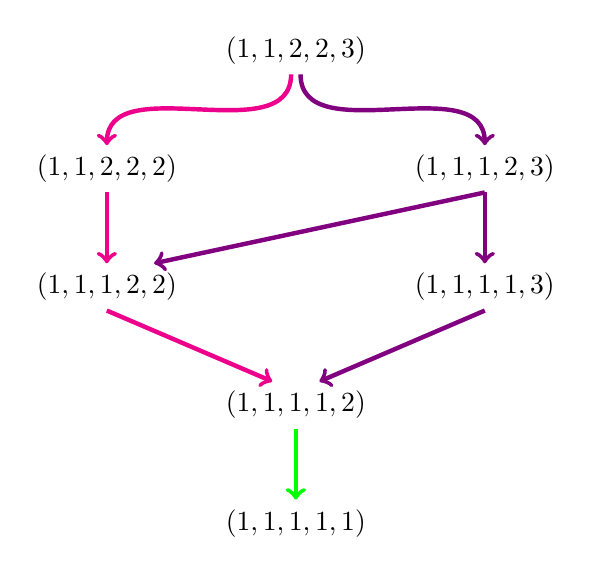
\begin{tikzpicture}[scale = 0.3]
    \node at (0,0) {$(1, 1, 1, 1, 1)$};

    \node at (0,5) {$(1, 1, 1, 1, 2)$};
        
    \node at (-8,10) {$(1, 1, 1, 2, 2)$};
    \node at (8,10)  {$(1, 1, 1, 1, 3)$};

    \node at (-8,15) {$(1, 1, 2, 2, 2)$};
    \node at (8,15)  {$(1, 1, 1, 2, 3)$};

    \node at (0,20) {$(1, 1, 2, 2, 3)$};

    \draw [->][out=-90,in=90, ultra thick] 
        [color=magenta](-0.2,19) to (-8,16);
    \draw [->][color=magenta, ultra thick]
        (-8,14) to (-8,11);
    \draw [->][color=magenta, ultra thick]
        (-8,9) to (-1,6);        

    \draw [->][out=-90,in=90, ultra thick] 
        [color=green](0,4) to (0,1);

    \draw [->][out=-90,in=90, ultra thick]
        [color=violet](0.2,19) to (8,16);
    \draw [->][color=violet, ultra thick]
        (8,14) to (-6,11);
    \draw [->][color=violet, ultra thick]
        (8,14) to (8,11);
    \draw [->][color=violet, ultra thick]
        (8,9) to (1,6);

\end{tikzpicture}
\end{center}
        \begin{center}
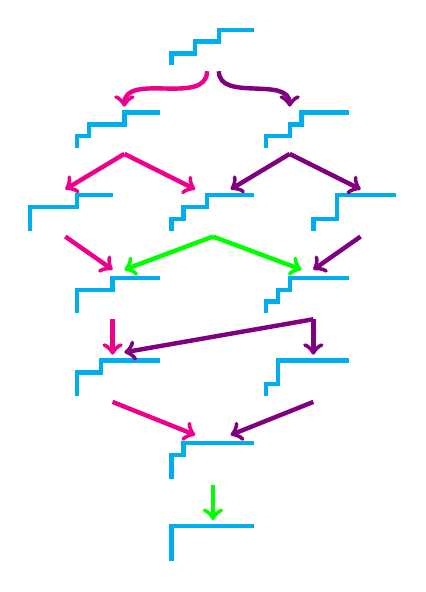
\begin{tikzpicture}[scale = 0.15]
    \draw [ultra thick, color = cyan] (0,0) -- (0,1)
        -- (0,2) -- (0,3) -- (1,3) -- (2,3) -- (3,3)
        -- (4,3) -- (5,3) -- (6,3) -- (7,3);

    \draw [ultra thick, color = cyan] (0,7) -- (0,8)
        -- (0,9) -- (1,9) -- (1,10) -- (2,10) -- (3,10)
        -- (4,10) -- (5,10) -- (6,10) -- (7,10);

    \draw [ultra thick, color = cyan] (-8,14) -- (-8,15)
        -- (-8,16) -- (-7,16) -- (-6,16) -- (-6,17) -- (-5,17)
        -- (-4,17) -- (-3,17) -- (-2,17) -- (-1,17);
        
    \draw [ultra thick, color = cyan] (8,14) -- (8,15)
        -- (9,15) -- (9,16) -- (9,17) -- (10,17)
        -- (11,17) -- (12,17) -- (13,17) -- (14,17)
        -- (15,17);

    \draw [ultra thick, color = cyan] (-8,21) -- (-8,22)
        -- (-8,23) -- (-7,23) -- (-6,23) -- (-5,23)
        -- (-5,24) -- (-4,24) -- (-3,24) -- (-2,24)
        -- (-1, 24);

    \draw [ultra thick, color = cyan] (8,21) -- (8,22)
        -- (9,22) -- (9,23) -- (10,23) -- (10,24) -- (11,24)
        -- (12,24) -- (13,24) -- (14,24) -- (15,24);

    \draw [ultra thick, color = cyan] (-12,28) -- (-12,29)
        -- (-12,30) -- (-11,30) -- (-10,30) -- (-9,30) -- (-8,30)
        -- (-8,31) -- (-7,31) -- (-6,31) -- (-5,31);

    \draw [ultra thick, color = cyan] (0,28) -- (0,29)
        -- (1,29) -- (1,30) -- (2,30) -- (3,30) -- (3,31)
        -- (4,31) -- (5,31) -- (6,31) -- (7,31);

    \draw [ultra thick, color = cyan] (12,28) -- (12,29)
        -- (13,29) -- (14,29) -- (14,30) -- (14,31) -- (15,31)
        -- (16,31) -- (17,31) -- (18,31) -- (19,31);

    \draw [ultra thick, color = cyan] (-8,35) -- (-8,36)
        -- (-7,36) -- (-7,37) -- (-6,37) -- (-5,37) -- (-4,37)
        -- (-4,38) -- (-3,38) -- (-2,38) -- (-1,38);

    \draw [ultra thick, color = cyan] (8,35) -- (8,36)
        -- (9,36) -- (10,36) -- (10,37) -- (11,37) -- (11,38)
        -- (12,38) -- (13,38) -- (14,38) -- (15,38);

    \draw [ultra thick, color = cyan] (0,42) -- (0,43)
        -- (1,43) -- (2,43) -- (2,44) -- (3,44) -- (4,44)
        -- (4,45) -- (5,45) -- (6,45) -- (7,45);

    \draw [->][out=-90,in=90, ultra thick] 
        [color=magenta](3,41.5) to (-4,38.5);
    \draw [->][color=magenta, ultra thick]
        (-4,34.5) to (-9,31.5);
    \draw [->][color=magenta, ultra thick]
        (-4,34.5) to (2,31.5);        
    \draw [->][color=magenta, ultra thick]
        (-9,27.5) to (-5,24.7);
    \draw [->][color=magenta, ultra thick]
        (-5,20.5) to (-5,17.5);
    \draw [->][color=magenta, ultra thick]
        (-5,13.5) to (2,10.7);

    \draw [->][color=green, ultra thick]
        (3.5,27.5) to (-4,24.7);
    \draw [->][color=green, ultra thick]
        (3.5,27.5) to (11,24.7);
    \draw [->][out=-90,in=90, ultra thick] 
        [color=green](3.5,6.5) to (3.5,3.5);

    \draw [->][out=-90,in=90, ultra thick]
        [color=violet](4,41.5) to (10,38.5);
    \draw [->][color=violet, ultra thick]
        (10,34.5) to (5,31.5);
    \draw [->][color=violet, ultra thick]
        (10,34.5) to (16,31.5);
    \draw [->][color=violet, ultra thick]
        (16,27.5) to (12,24.7);
    \draw [->][color=violet, ultra thick]
        (12,20.5) to (-4,17.7);
    \draw [->][color=violet, ultra thick]
        (12,20.5) to (12,17.5);
    \draw [->][color=violet, ultra thick]
        (12,13.5) to (5,10.7);

\end{tikzpicture}
\end{center}
    \end{center}
\end{example}

\begin{rem}
    ~
    \begin{itemize}
        \item $rot (rot^{-1}(P)) = rot^{-1}(rot(P)) = P$
        \item $rot(P)$ and $rot^{-1}(P)$ are always
            non-crossing partitions.
        \item If $P \in \mathcal{NC}_n$, then $rot^n(P) =
            rot^{-n}(P) = P$.
    \end{itemize}
\end{rem}

\begin{prop}
    $K (K (P)) = rot^{-1} (P)$.
\end{prop}

\begin{example}[$P = \{\{1, 6\}, \{2, 3, 5\}, \{4\}\}$]
    ~
    \begin{center}
        \begin{center}
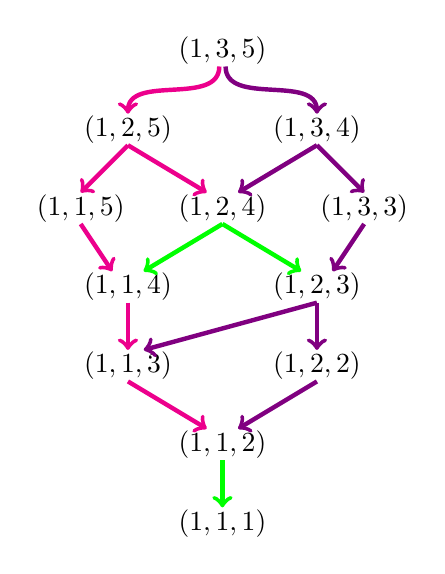
\begin{tikzpicture}[scale = 0.2]
    \node at (0,0) {$(1,1,1)$};

    \node at (0,5) {$(1,1,2)$};

    \node at (-6,10) {$(1,1,3)$};                
    \node at (6,10)  {$(1,2,2)$};

    \node at (-6,15) {$(1,1,4)$};
    \node at (6,15)  {$(1,2,3)$};

    \node at (-9,20) {$(1,1,5)$};
    \node at (0,20)  {$(1,2,4)$};
    \node at (9,20)  {$(1,3,3)$};

    \node at (-6,25) {$(1,2,5)$};
    \node at (6,25)  {$(1,3,4)$};

    \node at (0,30) {$(1,3,5)$};

    \draw [->][out=-90,in=90, ultra thick] 
        [color=magenta](-0.2,29) to (-6,26);
    \draw [->][color=magenta, ultra thick]
        (-6,24) to (-9,21);
    \draw [->][color=magenta, ultra thick]
        (-6,24) to (-1,21);        
    \draw [->][color=magenta, ultra thick]
        (-9,19) to (-7,16);
    \draw [->][color=magenta, ultra thick]
        (-6,14) to (-6,11);
    \draw [->][color=magenta, ultra thick]
        (-6,9) to (-1,6);

    \draw [->][color=green, ultra thick]
        (0,19) to (-5,16);
    \draw [->][color=green, ultra thick]
        (0,19) to (5,16);
    \draw [->][out=-90,in=90, ultra thick] 
        [color=green](0,4) to (0,1);

    \draw [->][out=-90,in=90, ultra thick]
        [color=violet](0.2,29) to (6,26);
    \draw [->][color=violet, ultra thick]
        (6,24) to (1,21);
    \draw [->][color=violet, ultra thick]
        (6,24) to (9,21);
    \draw [->][color=violet, ultra thick]
        (9,19) to (7,16);
    \draw [->][color=violet, ultra thick]
        (6,14) to (-5,11);
    \draw [->][color=violet, ultra thick]
        (6,14) to (6,11);
    \draw [->][color=violet, ultra thick]
        (6,9) to (1,6);

\end{tikzpicture}
\end{center}
          ~\\
          ~\\
    
        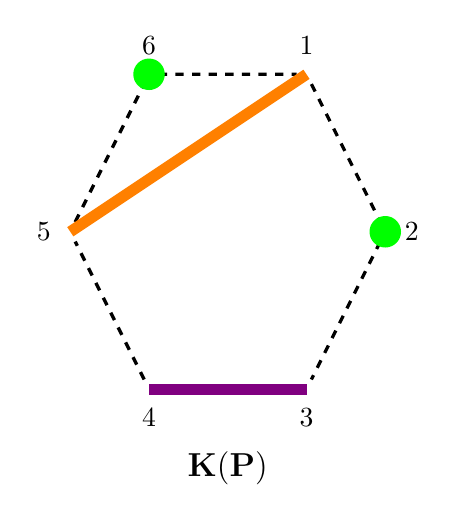
\begin{tikzpicture}[scale=1]
    \node at (3,0) {\large $\mathbf{K(P)}$};
    \node [label = above : {$1$}] (1)
        at (4,5) {};
    \node [label = right : {$2$}] (2)
        at (5,3) {};
    \node [label = below : {$3$}] (3)
        at (4,1) {};
    \node [label = below : {$4$}] (4)
        at (2,1) {};
    \node [label = left : {$5$}]  (5)
        at (1,3) {};
    \node [label = above : {$6$}] (6)
        at (2,5) {};
    \draw [dashed][very thick]
    (1) -- (2) -- (3) -- (4)
        -- (5) -- (6) -- (1);
    \draw [color = orange][line width = 4pt] 
        (4,5) -- (1,3);            
    \draw [color = violet][line width = 4pt] 
        (4,1) -- (2,1);
    \fill [color=green] (5,3) circle (0.2); 
    \fill [color=green] (2,5) circle (0.2);   
  \end{tikzpicture}
        \begin{center}
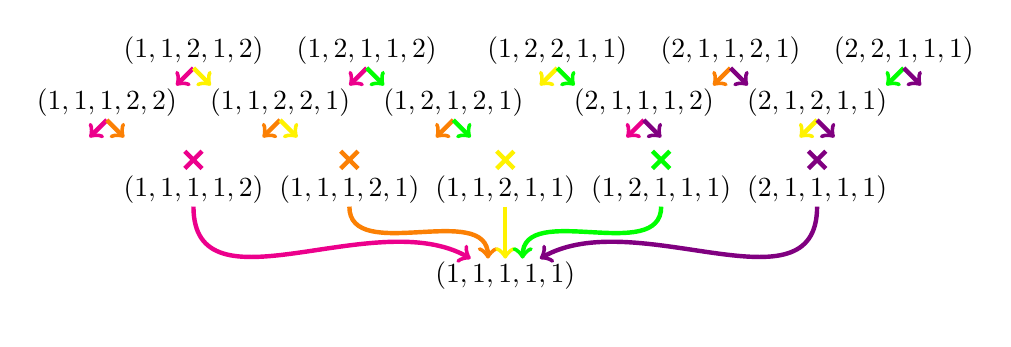
\begin{tikzpicture}[scale = 0.22]
    \node at (0,0) {$(1,1,1,1,1)$};

    \node at (-18,5) {$(1,1,1,1,2)$};
    \node at (-9,5)  {$(1,1,1,2,1)$};
    \node at (0,5)   {$(1,1,2,1,1)$};
    \node at (9,5)   {$(1,2,1,1,1)$};
    \node at (18,5)  {$(2,1,1,1,1)$};

    \node at (-23,10) {$(1,1,1,2,2)$};
    \node at (-18,13) {$(1,1,2,1,2)$};
    \node at (-13,10) {$(1,1,2,2,1)$};
    \node at (-8,13)  {$(1,2,1,1,2)$};
    \node at (-3,10)  {$(1,2,1,2,1)$};
    \node at (3,13)   {$(1,2,2,1,1)$};
    \node at (8,10)   {$(2,1,1,1,2)$};
    \node at (13,13)  {$(2,1,1,2,1)$};
    \node at (18,10)  {$(2,1,2,1,1)$};
    \node at (23,13)  {$(2,2,1,1,1)$};

    \draw [->][color=magenta, ultra thick]
        (-23,9) to (-24,8);
    \draw [->][color=magenta, ultra thick]
        (-18,12) to (-19,11);
    \draw [->][color=magenta, ultra thick]
        (-8,12) to (-9,11);
    \draw [->][color=magenta, ultra thick]
        (8,9) to (7,8);
    \draw[color=magenta, ultra thick]
        (-18.5,7.2) -- (-17.5,6.2);
    \draw[color=magenta, ultra thick]
        (-18.5,6.2) -- (-17.5,7.2);
    \draw [->][out=-90,in=150, ultra thick] 
        [color=magenta](-18,4) to (-2,1);

    \draw [->][color=brown!7!orange, ultra thick]
        (-23,9) to (-22,8);
    \draw [->][color=brown!7!orange, ultra thick]
        (-13,9) to (-14,8);
    \draw [->][color=brown!7!orange, ultra thick]
        (-3,9) to (-4,8);
    \draw [->][color=brown!7!orange, ultra thick]
        (13,12) to (12,11);
    \draw[color=brown!7!orange, ultra thick]
        (-9.5,7.2) -- (-8.5,6.2);
    \draw[color=brown!7!orange, ultra thick]
        (-9.5,6.2) -- (-8.5,7.2);
    \draw [->][out=-90,in=90, ultra thick]
        [color=brown!7!orange](-9,4) to (-1,1);

    \draw [->][color=yellow, ultra thick]
        (-18,12) to (-17,11); 
    \draw [->][color=yellow, ultra thick]
        (-13,9) to (-12,8); 
    \draw [->][color=yellow, ultra thick]
        (3,12) to (2,11); 
    \draw [->][color=yellow, ultra thick]
        (18,9) to (17,8); 
    \draw[color=yellow, ultra thick]
        (-0.5,7.2) -- (0.5,6.2);
    \draw[color=yellow, ultra thick]
        (-0.5,6.2) -- (0.5,7.2);
    \draw [->][out=-90,in=90, ultra thick] 
        [color=yellow](0,4) to (0,1);

    \draw [->][color = green,  ultra thick]
        (-8,12) to (-7,11);
    \draw [->][color=green, ultra thick]
        (-3,9) to (-2,8);
    \draw [->][color=green, ultra thick]
        (3,12) to (4,11);
    \draw [->][color=green, ultra thick]
        (23,12) to (22,11);
    \draw[color=green, ultra thick]
        (8.5,7.2) -- (9.5,6.2);
    \draw[color=green, ultra thick]
        (8.5,6.2) -- (9.5,7.2);
    \draw [->][out=-90,in=90, ultra thick]
        [color=green](9,4) to (1,1);

    \draw [->][color=violet, ultra thick]
        (8,9) to (9,8);
    \draw [->][color=violet, ultra thick]
        (13,12) to (14,11);
    \draw [->][color=violet, ultra thick]
        (18,9) to (19,8);
    \draw [->][color=violet, ultra thick]
        (23,12) to (24,11);
    \draw[color=violet, ultra thick]
        (17.5,7.2) -- (18.5,6.2);
    \draw[color=violet, ultra thick]
        (17.5,6.2) -- (18.5,7.2);
    \draw [->][out=-90,in=30, ultra thick] 
        [color=violet](18,4) to (2,1);

\end{tikzpicture}
\end{center}
    \end{center}
\end{example}